% ============================================================
%  CyberBattleSim-LLM Dataset Documentation
%  Thesis chapter / technical report
% ============================================================
\documentclass[11pt,a4paper]{article}

% --- Packages -----------------------------------------------
\usepackage[margin=2.5cm]{geometry}
\usepackage{microtype}
\usepackage{amsmath}
\usepackage{xcolor}
\usepackage{xspace}
\usepackage{booktabs}
\usepackage{tabularx}
\usepackage{tikz}
\usetikzlibrary{arrows.meta, positioning, fit, backgrounds}
\usepackage[colorlinks=true, linkcolor=blue!60!black,
            citecolor=blue!60!black, urlcolor=blue!60!black]{hyperref}
\usepackage[capitalise,noabbrev]{cleveref}
\usepackage[textsize=small]{todonotes}

% --- Custom commands ----------------------------------------
\newcommand{\CBS}{CyberBattleSim\xspace}
\newcommand{\CBSL}{CyberBattleSim-LLM\xspace}
\newcommand{\CAGE}{CAGE\xspace}
\newcommand{\CybORG}{CybORG\xspace}
\newcommand{\NSE}{NASimEmu\xspace}
\newcommand{\FARLAND}{FARLAND\xspace}
\newcommand{\NSG}{NetSecGame\xspace}

% ============================================================
\title{\textbf{CyberBattleSim-LLM: A Large-Scale LLM-Generated
       and LLM-Validated Dataset of Enterprise Network Attack
       Scenarios for Reinforcement Learning}}
\author{Ariel Zilbershteyin\\
        \small{ariel@prompt.security}}
\date{June 2026}
% ============================================================

\begin{document}
\maketitle
\tableofcontents
\newpage

% ------------------------------------------------------------
\section{Introduction}
\label{sec:intro}
% ------------------------------------------------------------

Autonomous cyber defense—the application of reinforcement learning (RL) to
network intrusion response—has attracted growing research interest as
enterprise networks become too large and fast-moving for purely human
defenders.  A central bottleneck for this research program is the
availability of \emph{training environments}: simulators that expose a
defender (or attacker) agent to diverse, realistic network topologies and
attack chains.  Without sufficient environmental diversity, RL agents
overfit to the handful of fixed scenarios bundled with a given simulator and
fail to generalize to unseen deployments.

Existing simulators each ship with only a small corpus of hand-crafted
scenarios.  \CBS~\cite{cyberbattlesim2021} provides three toy network graphs
plus one CTF-style example.  The \CAGE Challenges~\cite{cage2021} define a
single enterprise topology per challenge cycle.  \CybORG~\cite{cyborg2020}
exposes two fixed network layouts.  Manually designing hundreds of
internally-consistent, solvable scenarios---each with coordinated node
configurations, service vulnerabilities, credential chains, and lateral
movement paths---requires significant domain expertise and is essentially
intractable at scale.

This paper introduces the \CBSL dataset: \textbf{1,000 validated enterprise
network attack scenarios} generated entirely by a pipeline of specialist
large language model (LLM) agents and quality-filtered by a two-phase
automated validation system.  The dataset spans five distinct attack
families and four network sizes (Small, Medium, Large, XLarge), giving $5
\times 4 = 20$ scenario templates with 50 instances each ($40$ train $+$ $10$
test, a fixed 80/20 split).

Our key contributions are:
\begin{itemize}
    \item A \textbf{multi-agent LLM generation pipeline} with five specialist
          agents covering network topology, Linux services, Windows/Active
          Directory, credential chains, and lateral movement.
    \item A \textbf{two-phase validation framework}: Phase~1 applies 22
          deterministic static checks; Phase~2 combines BFS solvability
          evaluation (required solve rate $\geq 0.80$), a six-dimensional LLM
          quality evaluator (required score $\geq 8.0/10$), and an
          actor--critic repair loop of up to three rounds.
    \item The \CBSL \textbf{benchmark protocol}: standardized train/test
          splits, evaluation metrics, and suggested RL baselines to make
          results across papers directly comparable.
\end{itemize}

To the best of our knowledge, \CBSL is the only publicly released corpus of
network attack scenarios that is simultaneously LLM-generated,
LLM-validated, and parameterized across scale.

% ------------------------------------------------------------
\section{Background}
\label{sec:background}
% ------------------------------------------------------------

\paragraph{\CBS mechanics.}
\CBS~\cite{cyberbattlesim2021} represents an enterprise network as a directed
graph of \emph{nodes}, where each node runs one or more \emph{services} with
associated vulnerabilities.  Nodes hold \emph{credentials} that, once
discovered or stolen by an attacker, unlock lateral movement to adjacent
nodes.  An episode begins with the attacker controlling an \emph{entry node}
and ends when the attacker captures a designated \emph{flag node} (the
``crown jewel'').

\paragraph{Scenarios as YAML/Python configs.}
A \emph{scenario} is a YAML configuration file that is parsed into a Python
\texttt{NetworkX} graph.  The YAML encodes the node inventory, service
definitions, vulnerability parameters, initial credential distribution, and
reachability edges.  This design makes scenarios human-readable and
programmatically manipulable, which our pipeline exploits during repair.

\paragraph{Difficulty and scale variation.}
RL generalization requires agents trained on easy environments to transfer to
harder ones.  In network security, difficulty derives from graph diameter,
the number of credential-chain hops required to reach the flag, the density
of decoy services, and the size of the action space.  A corpus that
systematically varies network size—while holding attack-family constant—
provides a natural curriculum for progressively harder training.

% ------------------------------------------------------------
\section{Related Work}
\label{sec:related}
% ------------------------------------------------------------

\paragraph{\CBS~\cite{cyberbattlesim2021}.}
Microsoft's open-source simulator introduced the node-service-credential
abstraction used in this work.  Its bundled scenarios are small ($\leq 20$
nodes) and cover a single attacker model (random and ``Credential
Stealing'').  Our pipeline generates 1,000 scenarios that vary attack family
and scale while remaining compatible with the \CBS engine.

\paragraph{\CAGE Challenges~\cite{cage2021}.}
The TTCP \CAGE series released three successive challenges (2021--2023) with
increasingly complex blue-team tasks.  Each challenge defines a single
network layout; participants design agents for that layout alone.  No
multi-scenario corpus is released.

\paragraph{\CybORG~\cite{cyborg2020}.}
The DSTO/DST Group's \CybORG simulator uses a more faithful OS-level action
model (scanning, exploitation, privilege escalation) but ships with only two
network topologies.

\paragraph{\NSE~\cite{nasimu2023}.}
Janisch et al.\ present a network attack simulator that bridges simulation
and emulation, with procedurally generated topologies.  Scenario generation
is rule-based, not LLM-driven, and quality validation is limited to
graph-theoretic feasibility.

\paragraph{\FARLAND~\cite{farland2021}.}
Molina-Markham et al.\ propose a framework for autonomous network defense
with randomized network configurations.  Scenarios are parameterized by a
random seed with no semantic attack-family structure.

\paragraph{\NSG/PenGym~\cite{netsecgame2024}.}
NetSecGame and PenGym provide graph-based RL environments for penetration
testing.  Scenario corpora are small and manually crafted.

\paragraph{Contrast with \CBSL.}
None of the above works combines (a) LLM-based semantic scenario generation,
(b) automated multi-dimensional quality validation, (c) systematic
parameterization across both attack family and network scale, and (d) a
large, fixed train/test corpus.  \CBSL addresses all four dimensions.

% ------------------------------------------------------------
\section{Pipeline Architecture}
\label{sec:pipeline}
% ------------------------------------------------------------

The \CBSL generation pipeline operates in three phases illustrated in
\cref{fig:pipeline}.  An initial YAML configuration—specifying the attack
family and target network size—is handed to a squad of specialist LLM agents
that collaboratively author the scenario.  The draft then passes through two
validation phases before being written to disk as a finalized artifact.

\begin{figure}[h]
\centering
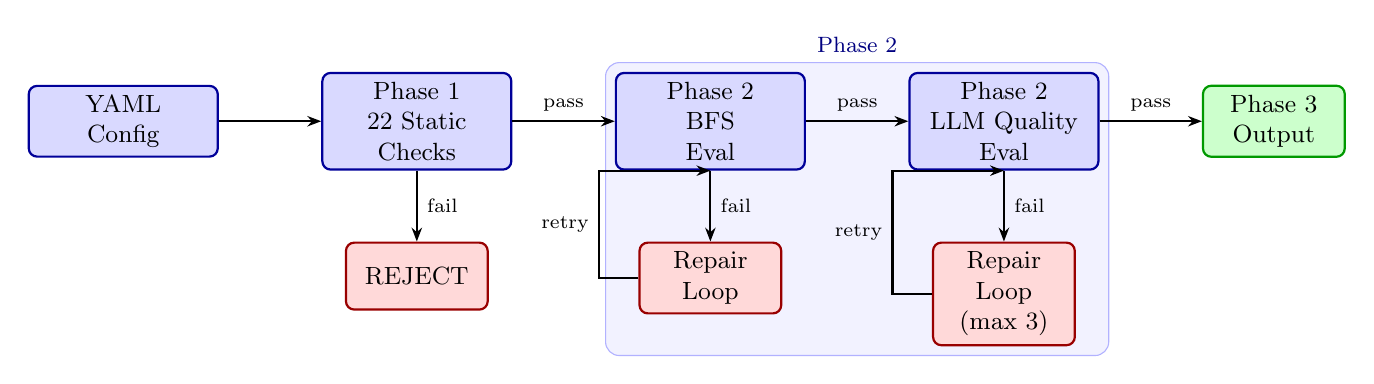
\begin{tikzpicture}[
    node distance = 0.9cm and 1.3cm,
    box/.style    = {rectangle, rounded corners=3pt, minimum width=2.4cm,
                     minimum height=0.85cm, align=center, font=\small,
                     draw, thick},
    phase/.style  = {box, fill=blue!15, draw=blue!60!black},
    pass/.style   = {box, fill=green!20, draw=green!60!black, minimum width=1.8cm},
    fail/.style   = {box, fill=red!15,  draw=red!60!black,   minimum width=1.8cm},
    arr/.style    = {-{Stealth[length=5pt]}, thick},
    labl/.style   = {font=\scriptsize, midway}
]

%% Row 1 – main happy path (left to right)
\node[phase]                    (yaml)   {YAML\\Config};
\node[phase, right=of yaml]     (p1)     {Phase 1\\22 Static\\Checks};
\node[phase, right=of p1]       (bfs)    {Phase 2\\BFS\\Eval};
\node[phase, right=of bfs]      (llmq)   {Phase 2\\LLM Quality\\Eval};
\node[pass,  right=of llmq]     (p3)     {Phase 3\\Output};

%% Failure nodes – below main path
\node[fail, below=0.9cm of p1]  (reject) {REJECT};
\node[fail, below=0.9cm of bfs] (repair1){Repair\\Loop};
\node[fail, below=0.9cm of llmq](repair2){Repair\\Loop\\(max 3)};

%% Main path arrows
\draw[arr] (yaml)  -- (p1);
\draw[arr] (p1)    -- node[labl,above]{pass} (bfs);
\draw[arr] (bfs)   -- node[labl,above]{pass} (llmq);
\draw[arr] (llmq)  -- node[labl,above]{pass} (p3);

%% Failure arrows
\draw[arr] (p1)   -- node[labl,right]{fail} (reject);
\draw[arr] (bfs)  -- node[labl,right]{fail} (repair1);
\draw[arr] (llmq) -- node[labl,right]{fail} (repair2);

%% Repair loops back to BFS / LLM eval
\draw[arr] (repair1.west) -- ++(-0.5,0) |- (bfs.south)
    node[pos=0.25, font=\scriptsize, left]{retry};
\draw[arr] (repair2.west) -- ++(-0.5,0) |- (llmq.south)
    node[pos=0.25, font=\scriptsize, left]{retry};

%% Phase background shading
\begin{pgfonlayer}{background}
    \node[draw=blue!30, fill=blue!5, rounded corners=5pt,
          fit=(bfs)(repair1)(repair2)(llmq),
          label={[blue!50!black, font=\footnotesize]above:Phase 2}] {};
\end{pgfonlayer}

\end{tikzpicture}
\caption{Overview of the three-phase \CBSL generation and validation pipeline.
         Blue boxes denote pipeline stages; green denotes the successful
         output path; red denotes rejection or repair.}
\label{fig:pipeline}
\end{figure}

\subsection{Specialist LLM Agents}
\label{sec:agents}

Scenario generation is distributed across five specialist agents, each
responsible for a semantically coherent sub-domain:

\begin{description}
    \item[$S_{\text{Network}}$] Designs the overall network topology:
          node inventory, subnet structure, inter-node reachability edges, and
          entry/exit points.  Ensures the graph is connected and that the
          attacker has a viable path from the entry node to the flag.

    \item[$S_{\text{Linux}}$] Populates Linux-based nodes with realistic
          service stacks (e.g., SSH, Apache, PostgreSQL, Redis) and
          corresponding CVE-class vulnerabilities.  Calibrates exploit
          difficulty to the target network size.

    \item[$S_{\text{Windows}}$] Configures Windows and Active Directory nodes:
          domain controllers, file servers, IIS, WinRM, LDAP, and
          Kerberoastable service accounts.  Models privilege escalation paths
          within the Windows trust model.

    \item[$S_{\text{Identity}}$] Constructs credential chains: which
          credentials live on which nodes, which vulnerabilities expose which
          credentials, and which credential-to-node mappings enable lateral
          movement.  Ensures no ``orphan'' credentials exist.

    \item[$S_{\text{Lateral}}$] Validates and augments lateral movement
          paths.  Ensures the attack graph contains at least one end-to-end
          chain and that the chain difficulty is commensurate with the target
          complexity level.
\end{description}

The agents operate sequentially with each agent's output feeding the next.
A meta-agent orchestrates the squad, resolves conflicts (e.g., a credential
$S_{\text{Identity}}$ places on a node that $S_{\text{Network}}$ declared
unreachable), and merges the outputs into a single candidate YAML.

\subsection{Phase 1: Static Validation (22 Checks)}
\label{sec:phase1}

Before any dynamic evaluation, the candidate YAML is subjected to 22
deterministic static checks organized into seven categories (see
\cref{app:checks} for the full list):

\begin{enumerate}
    \item \textbf{Schema validity} — all required YAML fields are present and
          correctly typed.
    \item \textbf{Graph connectivity} — the reachability graph is weakly
          connected; no isolated nodes.
    \item \textbf{Credential reachability} — every credential referenced in a
          lateral-move edge is discoverable from at least one reachable
          vulnerability.
    \item \textbf{Exploit-to-credential mapping} — every vulnerability payload
          references a credential that exists in the scenario.
    \item \textbf{Topology balance} — service counts and node degrees fall
          within the bounds for the declared network size.
    \item \textbf{Flag node reachability} — the flag node is reachable from
          the entry node via some sequence of credential-unlock steps.
    \item \textbf{Structural sanity} — no self-loops, no duplicate node IDs,
          no negative reward values, no missing service ports.
\end{enumerate}

A scenario that fails any Phase~1 check is \emph{immediately rejected}; the
pipeline does not attempt repair at this stage because static failures
typically indicate a fundamental structural error that the repair loop cannot
reliably correct without regenerating large portions of the scenario.

\subsection{Phase 2: Dynamic Evaluation and Repair}
\label{sec:phase2}

\paragraph{BFS solvability.}
A breadth-first search (BFS) attacker—an oracle agent that always takes the
locally optimal credential-stealing or service-exploitation action—attempts
to reach the flag node across multiple random seeds.  A scenario passes BFS
evaluation if its \emph{solve rate} (fraction of seeds where the attacker
reaches the flag within a budget of $T$ steps) is $\geq 0.80$.  This
threshold ensures that RL agents will receive a learning signal: if even an
oracle solver struggles, the scenario is either over-constrained or
incorrectly wired.

\paragraph{LLM quality evaluation.}
Scenarios passing BFS evaluation are scored by a separate LLM evaluator on
six dimensions, each rated 0--10:

\begin{itemize}
    \item \textbf{Realism} — do the node types, service stacks, and credential
          patterns resemble real enterprise deployments?
    \item \textbf{Coherence} — is the scenario internally consistent (e.g., a
          Windows-only subnet does not suddenly expose a Linux cron-job
          vulnerability)?
    \item \textbf{Difficulty} — is the estimated attacker effort appropriate
          for the declared network size?
    \item \textbf{Completeness} — are all nodes purposeful; are there no
          obvious gaps in the attack chain?
    \item \textbf{Diversity} — does the scenario offer distinct attack sub-paths
          rather than a single linear chain?
    \item \textbf{Exploitability} — are the vulnerability types and CVSS scores
          plausible and consistent with current threat intelligence?
\end{itemize}

A scenario must achieve a mean score of $\geq 8.0/10$ to pass.

\paragraph{Actor--critic repair loop.}
Scenarios failing either the BFS or LLM quality threshold enter an
\emph{actor--critic} repair loop.  An \emph{actor} LLM receives the
candidate YAML together with the failure report and proposes targeted edits
(e.g., adding a missing credential, rewiring an unreachable subnet, replacing
an implausible service).  A \emph{critic} LLM then reviews the proposed edits
for consistency before they are applied.  The repaired scenario is
re-evaluated from the failed phase.  The loop runs for at most three rounds;
scenarios still failing after round three are discarded.

\subsection{Phase 3: Artifact Packaging}
\label{sec:phase3}

Scenarios passing Phase~2 are written to disk as versioned YAML files and
indexed in a scenario manifest.  The manifest records the template name,
network size, attack family, BFS solve rate, LLM quality score, number of
repair rounds needed, and a SHA-256 content hash.  A summary HTML report is
generated per template showing pass/fail counts, score distributions, and
repair-round histograms.

% ------------------------------------------------------------
\section{Scenario Design}
\label{sec:scenarios}
% ------------------------------------------------------------

\subsection{Dataset Composition}

\Cref{tab:composition} shows the number of validated scenarios per attack
family and network size.  The dataset totals 1,000 scenarios across 20
templates.

\begin{table}[h]
\centering
\caption{Dataset composition: number of validated scenarios per attack
         family and network size (50 per cell = 40 train + 10 test).}
\label{tab:composition}
\begin{tabularx}{\linewidth}{@{} l *{4}{>{\centering\arraybackslash}X} r @{}}
\toprule
\textbf{Attack Family}
    & \textbf{Small} & \textbf{Medium}
    & \textbf{Large} & \textbf{XLarge}
    & \textbf{Total} \\
\midrule
Perimeter $\to$ Domain Escalation    & 50 & 50 & 50 & 50 & 200 \\
Branch $\to$ HQ Lateral Movement     & 50 & 50 & 50 & 50 & 200 \\
CI/CD $\to$ Production Compromise    & 50 & 50 & 50 & 50 & 200 \\
Cloud $\to$ Corp Identity Pivot      & 50 & 50 & 50 & 50 & 200 \\
Hybrid Enterprise Crown Jewels       & 50 & 50 & 50 & 50 & 200 \\
\midrule
\textbf{Total}                       & 250 & 250 & 250 & 250 & \textbf{1000} \\
\bottomrule
\end{tabularx}
\end{table}

\subsection{Attack Families}

\paragraph{Perimeter $\to$ Domain Escalation.}
Models the classic internet-facing-service-to-Active-Directory attack chain.
The attacker exploits a vulnerable DMZ service (e.g., web application, VPN
concentrator, Exchange) to gain an initial foothold, then pivots inward via
credential theft and Kerberoasting to compromise the domain controller.
Nodes include DMZ web servers, reverse proxies, a Windows domain controller,
and internal workstations.  The attacker objective is \texttt{DCSync} access
to the domain controller.

\paragraph{Branch $\to$ HQ Lateral Movement.}
Represents an attacker who compromises a lightly-secured branch office and
uses site-to-site VPN trust relationships to reach headquarters systems.
Node types emphasize remote-access gateways, file-share servers, and
heterogeneous branch endpoints.  Credential chains span site boundaries,
requiring the attacker to discover both local branch credentials and HQ
domain credentials.  The flag is a sensitive HQ database server.

\paragraph{CI/CD $\to$ Production Compromise.}
Captures software supply-chain attacks in which the adversary targets the
build-and-deploy pipeline to inject malicious artifacts into production.
Scenarios include Jenkins/GitHub Actions runners, artifact registries, and
Kubernetes-based production clusters.  The attacker must chain together
source-code repository access, build-server compromise, and registry
credential theft before reaching the production workload flag.

\paragraph{Cloud $\to$ Corp Identity Pivot.}
Models hybrid-cloud identity attacks in which over-privileged cloud IAM
roles or misconfigured federated identity providers allow an attacker who
controls a cloud workload to pivot into the on-premises corporate network.
Node types mix AWS/GCP compute instances, IAM role nodes, SAML identity
providers, and on-premises Active Directory.  The attacker objective is to
escalate from a cloud-resident shell to on-premises domain admin.

\paragraph{Hybrid Enterprise Crown Jewels.}
A composite attack family combining elements of all four preceding families.
Scenarios feature large, multi-segment networks (DMZ, cloud, branch, HQ)
with multiple potential attack paths to a single high-value target (the
``crown jewel''), such as a financial database or executive workstation.
This family is designed to stress-test RL agents on long-horizon planning
with many available sub-goals.

\subsection{Network Size Parameters}

\begin{center}
\begin{tabular}{@{}lcc@{}}
\toprule
\textbf{Size} & \textbf{Nodes} & \textbf{Services / Node} \\
\midrule
Small   & 5--10   & 2--4 \\
Medium  & 10--20  & 3--5 \\
Large   & 20--35  & 4--6 \\
XLarge  & 35--60  & 5--8 \\
\bottomrule
\end{tabular}
\end{center}

These ranges are enforced by Phase~1 topology balance checks.  The upper
bound on XLarge scenarios was chosen so that BFS evaluation remains
computationally tractable within the pipeline's time budget.

% ------------------------------------------------------------
\section{Validation and Quality Metrics}
\label{sec:validation}
% ------------------------------------------------------------

\subsection{Phase 1 Static Check Results}

The 22 static checks are organized into the seven categories described in
\cref{sec:phase1} and enumerated fully in \cref{app:checks}.
\todo{PLACEHOLDER: add overall Phase 1 pass rate (scenarios passing all 22
checks on first attempt) after pipeline completes.}
\todo{PLACEHOLDER: report which check category causes the most first-attempt
failures.}

\subsection{BFS Solvability Results}

\Cref{tab:bfs} reports the BFS solve rate, pass/total count, and mean
repair rounds needed for each of the 20 scenario templates.  All reported
figures are computed over the finalized dataset (post-repair).

\begin{table}[h]
\centering
\caption{BFS solvability statistics per scenario template.  ``Passed/Total''
         is the number of generated candidates that survived all phases over
         the total number generated to achieve the 50-scenario target.
         ``Rounds'' is the mean number of repair rounds across all repaired
         candidates.}
\label{tab:bfs}
\small
\begin{tabularx}{\linewidth}{@{} l l
    >{\centering\arraybackslash}X
    >{\centering\arraybackslash}X
    >{\centering\arraybackslash}X @{}}
\toprule
\textbf{Family} & \textbf{Size}
    & \textbf{BFS Solve Rate}
    & \textbf{Passed / Total}
    & \textbf{Mean Rounds} \\
\midrule
Perimeter $\to$ Domain  & Small   & \todo{xx} & \todo{xx/yy} & \todo{x.x} \\
Perimeter $\to$ Domain  & Medium  & \todo{xx} & \todo{xx/yy} & \todo{x.x} \\
Perimeter $\to$ Domain  & Large   & \todo{xx} & \todo{xx/yy} & \todo{x.x} \\
Perimeter $\to$ Domain  & XLarge  & \todo{xx} & \todo{xx/yy} & \todo{x.x} \\
\midrule
Branch $\to$ HQ         & Small   & \todo{xx} & \todo{xx/yy} & \todo{x.x} \\
Branch $\to$ HQ         & Medium  & \todo{xx} & \todo{xx/yy} & \todo{x.x} \\
Branch $\to$ HQ         & Large   & \todo{xx} & \todo{xx/yy} & \todo{x.x} \\
Branch $\to$ HQ         & XLarge  & \todo{xx} & \todo{xx/yy} & \todo{x.x} \\
\midrule
CI/CD $\to$ Prod        & Small   & \todo{xx} & \todo{xx/yy} & \todo{x.x} \\
CI/CD $\to$ Prod        & Medium  & \todo{xx} & \todo{xx/yy} & \todo{x.x} \\
CI/CD $\to$ Prod        & Large   & \todo{xx} & \todo{xx/yy} & \todo{x.x} \\
CI/CD $\to$ Prod        & XLarge  & \todo{xx} & \todo{xx/yy} & \todo{x.x} \\
\midrule
Cloud $\to$ Corp        & Small   & \todo{xx} & \todo{xx/yy} & \todo{x.x} \\
Cloud $\to$ Corp        & Medium  & \todo{xx} & \todo{xx/yy} & \todo{x.x} \\
Cloud $\to$ Corp        & Large   & \todo{xx} & \todo{xx/yy} & \todo{x.x} \\
Cloud $\to$ Corp        & XLarge  & \todo{xx} & \todo{xx/yy} & \todo{x.x} \\
\midrule
Hybrid Crown Jewels     & Small   & \todo{xx} & \todo{xx/yy} & \todo{x.x} \\
Hybrid Crown Jewels     & Medium  & \todo{xx} & \todo{xx/yy} & \todo{x.x} \\
Hybrid Crown Jewels     & Large   & \todo{xx} & \todo{xx/yy} & \todo{x.x} \\
Hybrid Crown Jewels     & XLarge  & \todo{xx} & \todo{xx/yy} & \todo{x.x} \\
\bottomrule
\end{tabularx}
\end{table}

\subsection{LLM Quality Evaluation Results}

\Cref{tab:quality} reports mean LLM quality scores per attack family across
all size variants.

\begin{table}[h]
\centering
\caption{Mean LLM quality scores per attack family (scale 0--10 per
         dimension; threshold $\geq 8.0$ mean required to pass).}
\label{tab:quality}
\small
\begin{tabularx}{\linewidth}{@{} l
    >{\centering\arraybackslash}X
    >{\centering\arraybackslash}X
    >{\centering\arraybackslash}X
    >{\centering\arraybackslash}X
    >{\centering\arraybackslash}X
    >{\centering\arraybackslash}X
    >{\centering\arraybackslash}X @{}}
\toprule
\textbf{Family}
    & \textbf{Real.}
    & \textbf{Coh.}
    & \textbf{Diff.}
    & \textbf{Comp.}
    & \textbf{Div.}
    & \textbf{Expl.}
    & \textbf{Mean} \\
\midrule
Perimeter $\to$ Domain
    & \todo{x.x} & \todo{x.x} & \todo{x.x}
    & \todo{x.x} & \todo{x.x} & \todo{x.x} & \todo{x.x} \\
Branch $\to$ HQ
    & \todo{x.x} & \todo{x.x} & \todo{x.x}
    & \todo{x.x} & \todo{x.x} & \todo{x.x} & \todo{x.x} \\
CI/CD $\to$ Prod
    & \todo{x.x} & \todo{x.x} & \todo{x.x}
    & \todo{x.x} & \todo{x.x} & \todo{x.x} & \todo{x.x} \\
Cloud $\to$ Corp
    & \todo{x.x} & \todo{x.x} & \todo{x.x}
    & \todo{x.x} & \todo{x.x} & \todo{x.x} & \todo{x.x} \\
Hybrid Crown Jewels
    & \todo{x.x} & \todo{x.x} & \todo{x.x}
    & \todo{x.x} & \todo{x.x} & \todo{x.x} & \todo{x.x} \\
\midrule
\textbf{All families}
    & \todo{x.x} & \todo{x.x} & \todo{x.x}
    & \todo{x.x} & \todo{x.x} & \todo{x.x} & \todo{x.x} \\
\bottomrule
\end{tabularx}
\end{table}

% ------------------------------------------------------------
\section{Benchmark Protocol}
\label{sec:benchmark}
% ------------------------------------------------------------

\paragraph{Train/test split.}
Each of the 20 templates contributes 40 training scenarios and 10 test
scenarios (80/20 split), yielding 800 training and 200 test scenarios in
total.  The split is fixed and provided as a manifest file in the dataset
release.  \textbf{No scenario appears in both splits}: the 50 instances per
template were generated independently, with distinct random seeds and
independent LLM sampling runs.

\paragraph{Evaluation metrics.}
We recommend three primary metrics for RL agent evaluation:
\begin{itemize}
    \item \textbf{Cumulative reward} — total undiscounted reward accumulated
          over an episode, normalized by the maximum possible reward for the
          scenario.
    \item \textbf{Steps to flag} — number of environment steps taken by the
          agent before capturing the flag node, measured only on successful
          episodes.  Lower is better.
    \item \textbf{Success rate} — fraction of test episodes in which the agent
          captures the flag within a step budget of $T = 500$ steps.
\end{itemize}

Separate leaderboard tracks are defined for Small/Medium (in-distribution
generalization) and Large/XLarge (out-of-distribution scale transfer).

\paragraph{Suggested baselines.}
For Small and Medium scenarios, we suggest DQN~\cite{cyberbattlesim2021},
PPO, and A2C as standard baselines using the action-space wrapper provided
with the dataset.  For Large and XLarge scenarios, transfer-learning
experiments (pre-train on Small/Medium, fine-tune on Large/XLarge) are the
primary research question and should be reported in addition to
from-scratch training results.

% ------------------------------------------------------------
\section{Limitations}
\label{sec:limitations}
% ------------------------------------------------------------

\paragraph{LLM hallucination.}
The quality evaluator is itself an LLM and may assign high scores to
scenarios that are superficially plausible but technically incorrect (e.g.,
a CVE assigned to the wrong operating system version).  Human red-team
validation of a random sample is recommended before using the dataset for
security-sensitive research.

\paragraph{BFS is a weak oracle.}
BFS traversal represents an omniscient attacker with perfect knowledge of the
credential graph.  Real RL agents operate under partial observability and may
find the effective difficulty of a scenario significantly higher or lower
than the BFS solve rate implies.  The BFS threshold ($\geq 0.80$) is a
necessary but not sufficient condition for RL learnability.

\paragraph{No adversarial stress-testing.}
Scenarios are parameterized for diversity and realism but have not been
subjected to adversarial perturbation (e.g., systematically inserting
credential dead-ends or unreachable flag nodes that evade static checks).
RL agents trained on this corpus may be brittle to such adversarial
modifications.

\paragraph{Credential reuse patterns.}
The identity specialist agent tends to produce credential chains in which a
single high-privilege credential unlocks multiple lateral-movement edges.
This pattern, while common in real-world breaches, may be more convenient
than typical enterprise deployments warrant.  Future versions of the pipeline
should enforce stricter constraints on credential fan-out.

\paragraph{No emulation validation.}
Scenarios are validated only within the \CBS simulator.  No emulation or
live-network replay is performed to confirm that the described services and
vulnerabilities are exploitable in practice.

% ------------------------------------------------------------
% Bibliography
% ------------------------------------------------------------
\bibliographystyle{plain}
\bibliography{refs}

% ============================================================
\appendix
% ============================================================

\section{Quality Evaluator Prompt Template}
\label{app:prompt}

The following prompt is sent verbatim to the LLM quality evaluator for each
candidate scenario.  The placeholder \texttt{\{YAML\}} is replaced with the
full scenario YAML text.

\begin{verbatim}
You are a senior penetration tester and enterprise network architect.
You will evaluate a CyberBattleSim scenario YAML for quality across
six dimensions. Read the scenario carefully, then provide a JSON
response with the following structure:

{
  "realism":        <0-10>,
  "coherence":      <0-10>,
  "difficulty":     <0-10>,
  "completeness":   <0-10>,
  "diversity":      <0-10>,
  "exploitability": <0-10>,
  "reasoning": "<brief justification for each score>",
  "repair_suggestions": "<specific actionable fixes if score < 8>"
}

Scoring rubric:
- realism (0-10): Do node types, service stacks, and credential
  patterns match real enterprise deployments? Penalize fantasy
  services or impossible CVE assignments.
- coherence (0-10): Is the scenario internally consistent? Penalize
  mixed OS environments without explanation, unreachable subnets
  that are referenced, or credentials that no vulnerability exposes.
- difficulty (0-10): Is attacker effort appropriate for the declared
  network size? Small networks should be solvable in <50 steps;
  XLarge in 100-400 steps.
- completeness (0-10): Are all nodes purposeful? Is there a clear
  end-to-end attack path from entry node to flag node?
- diversity (0-10): Does the scenario offer multiple distinct attack
  sub-paths, or is it a single linear chain?
- exploitability (0-10): Are vulnerability types (service name,
  exploit type, CVSS score) plausible and consistent with current
  threat intelligence?

The scenario YAML is enclosed below.
---
{YAML}
---
Respond with valid JSON only. Do not add prose outside the JSON block.
\end{verbatim}

% ------------------------------------------------------------
\section{Complete List of 22 Static Validation Checks}
\label{app:checks}
% ------------------------------------------------------------

\begin{enumerate}
    \item \textbf{YAML schema validity} — all top-level keys (\texttt{nodes},
          \texttt{entry\_node}, \texttt{flag\_node}, \texttt{credenials}) are
          present and non-empty.
    \item \textbf{Node ID uniqueness} — no two nodes share the same
          \texttt{id} field.
    \item \textbf{Entry node exists} — \texttt{entry\_node} references a node
          ID present in \texttt{nodes}.
    \item \textbf{Flag node exists} — \texttt{flag\_node} references a node
          ID present in \texttt{nodes}.
    \item \textbf{Entry $\neq$ flag} — \texttt{entry\_node} and
          \texttt{flag\_node} are distinct.
    \item \textbf{No isolated nodes} — every node has at least one incoming
          or outgoing reachability edge.
    \item \textbf{Graph weak connectivity} — the reachability graph (ignoring
          edge direction) is connected.
    \item \textbf{Entry node reachability} — the entry node can reach at
          least one other node via directed reachability edges.
    \item \textbf{Flag node reachability} — the flag node is reachable from
          the entry node via some directed path.
    \item \textbf{Service schema} — every service definition contains
          \texttt{name}, \texttt{port}, and \texttt{protocol} fields.
    \item \textbf{Vulnerability schema} — every vulnerability contains
          \texttt{name}, \texttt{type}, \texttt{outcome}, and \texttt{reward}.
    \item \textbf{Positive rewards} — all vulnerability \texttt{reward} values
          are $\geq 0$.
    \item \textbf{Credential schema} — every credential entry contains
          \texttt{name}, \texttt{username}, and \texttt{password} (or key
          reference).
    \item \textbf{No orphan credentials} — every credential name referenced
          in a lateral-move edge exists in the credential store.
    \item \textbf{Exploit-to-credential mapping} — every vulnerability whose
          \texttt{outcome} type is \texttt{credential\_access} references a
          credential that exists.
    \item \textbf{Credential-to-node mapping} — every credential used in a
          lateral-move edge maps to exactly one target node.
    \item \textbf{No duplicate services per node} — within a single node, no
          two services share the same \texttt{port}/\texttt{protocol} pair.
    \item \textbf{Node count within bounds} — the number of nodes falls within
          the declared size range (see \cref{sec:scenarios}).
    \item \textbf{Service count within bounds} — the mean services-per-node
          count is within the declared size range.
    \item \textbf{No self-loop edges} — no node lists itself as a reachability
          target.
    \item \textbf{Port number validity} — all port numbers are integers in
          $[1, 65535]$.
    \item \textbf{Lateral-move chain length} — the shortest credential-unlock
          path from entry to flag has length $\geq 1$ (the flag is not
          directly accessible from the entry node without at least one
          intermediate credential step).
\end{enumerate}

% ------------------------------------------------------------
\section{Example Scenario YAML Snippet}
\label{app:yaml}
% ------------------------------------------------------------

The following is an abbreviated YAML excerpt from a \emph{Small} instance of
the \emph{Perimeter $\to$ Domain Escalation} template.  Fields irrelevant to
illustrating the structure have been omitted.

\begin{verbatim}
scenario_id: perimeter_domain_small_0042
attack_family: perimeter_domain_escalation
size: small
entry_node: dmz_webserver
flag_node: dc01

nodes:
  - id: dmz_webserver
    os: linux
    services:
      - name: apache_httpd
        port: 443
        protocol: https
      - name: tomcat
        port: 8080
        protocol: http
    vulnerabilities:
      - name: CVE-2021-41773_path_traversal
        type: remote_code_execution
        outcome: credential_access
        credential: svc_deploy_key
        reward: 10
        cvss: 9.8

  - id: internal_jumphost
    os: linux
    services:
      - name: openssh
        port: 22
        protocol: ssh
    vulnerabilities:
      - name: sudo_token_reuse
        type: privilege_escalation
        outcome: credential_access
        credential: domain_svc_account
        reward: 15
        cvss: 7.4

  - id: dc01
    os: windows
    services:
      - name: ldap
        port: 389
        protocol: ldap
      - name: kerberos
        port: 88
        protocol: kerberos
    vulnerabilities:
      - name: kerberoast_svc_account
        type: credential_access
        outcome: flag
        credential: domain_admin
        reward: 100
        cvss: 6.5

credentials:
  - name: svc_deploy_key
    username: deploy
    password: "REDACTED"
  - name: domain_svc_account
    username: svc_backup
    password: "REDACTED"
  - name: domain_admin
    username: Administrator
    password: "REDACTED"

reachability:
  - from: dmz_webserver
    to: internal_jumphost
    via: svc_deploy_key
  - from: internal_jumphost
    to: dc01
    via: domain_svc_account
\end{verbatim}

\end{document}
